\section{The \proj framework}

Our proposed framework, \proj, adopts a retrieval-and-reasoning pipeline for KG-based RAG. Specifically, given a query $q$, \proj first extracts a subgraph $\gG_q\subset \gG$ that represents predicted relevant knowledge, and then LLMs generate the response by reasoning over $\gG_q$. While some existing works adopt a similar pipeline~\citep{zhang2022subgraph, luo2024rog, wu2023retrieve, wen2023mindmap}, our approach is novel in addressing three key challenges: First, the extracted subgraph $\gG_q$ is designed to comprehensively cover the relevant evidence for answering $q$, while adhering to a size constraint $K$, which can be adjusted according to the capacity of the downstream LLM. Second, the extraction of $\gG_q$ is highly efficient and scalable. Third, we employ tailored prompting to guide the LLM in reasoning over $\gG_q$ and generating a well-grounded answer with explanations.

\subsection{Efficient, Flexible and Expressive Subgraph Retrieval}
\label{sec:retriever}

\textbf{Problem Reduction} We formulate the subgraph retrieval problem and reduce it to an efficiently solvable problem. An LLM models $\mathbb{P}(\cdot | \gG_q, q)$ that takes queries and evidence subgraphs. Given a query $q$ and its answer $\mathcal{A}_{q}$, the best subgraph evidence for this LLM is denoted as $\gG_q^* = \argmax_{\gG_q\subseteq \gG} \mathbb{P}(\mathcal{A}_{q}\mid \gG_q, q)$. However, solving this problem is impossible as it requires the knowledge of $\mathcal{A}_{q}$. Instead, we aim to learn a subgraph retriever that generalizes to unseen future queries. 

Specifically, let the subgraph retriever be a distribution $\mathbb{Q}_{\theta}(\cdot | q, \gG)$ over the subgraph space of the KG, where $\theta$ denotes the parameters. Given a training set of question-answer pairs $\mathcal{D}$, the subgraph retriever learning problem can be formulated as the following problem: 
\begin{align} \label{eq:subgraph-retrieval}
    \max_{\theta } \; \mathbb{E}_{(q, \mathcal{A}_{q})\sim \mathcal{D}, \gG_q\sim \mathbb{Q}_{\theta}(\gG_q \mid q, \gG)}\;\mathbb{P}(\mathcal{A}_{q}\mid \gG_q, q).
\end{align}
This problem is hard to solve due to the complexity of the LLM ($\mathbb{P}$). Evaluating $\mathbb{P}(\mathcal{A}_{q}\mid \gG_q, q)$ requires the LLM to generate the particular answer $\mathcal{A}_{q}$, which can be costly and is only applicable to grey/white-box LLMs with accessible output logits, let alone the non-computable gradient $\frac{d\mathbb{P}}{d \gG_q}$.

To solve the problem in Eq.~\ref{eq:subgraph-retrieval}, we adopt the following strategy. If we know the optimal subgraph $\gG_q^*$, the maximum likelihood estimation (MLE) principle can be leveraged to train the retriever 
$\max_{\theta } \; \mathbb{E}_{(q, \mathcal{A}_{q})\sim \mathcal{D}}\;\mathbb{Q}_{\theta}(\gG_q^*\mid \gG, q)$. However, getting $\gG_q^*$ for an even known question-answer pair $(q,\mathcal{A}_q)$ is computationally hard and LLM-dependent. Instead, we use $(q,\mathcal{A}_q)$ to construct surrogate subgraph evidence with heuristics $\tilde{\gG}(q,\mathcal{A}_q)$ and train the retriever based on MLE:
\begin{align} \label{eq:MLE}
    \max_{\theta } \; \mathbb{E}_{(q, \mathcal{A}_{q})\sim \mathcal{D}}\;\mathbb{Q}_{\theta}(\tilde{\gG}_q\mid \gG, q), \quad \text{where $\tilde{\gG}_q=\tilde{\gG}(q,\mathcal{A}_q)$.}
\end{align}
An example $\tilde{\gG}_q$ is the shortest paths between the topic entities $\gT_q$ and answer entities $\gA_q$. Eq.~\ref{eq:MLE} is conceptually similar to the weak supervision in~\citet{zhang2022subgraph}. However, the formulation in Eq.~\ref{eq:MLE} indicates that the sampled subgraph does not necessarily follow a fixed type like path. Instead, the retriever distribution $\mathbb{Q}_{\theta}$ can by construction factorize into a product of distributions over triples, allowing efficient training and inference, flexible subgraph forms, and adjustable subgraph sizes.

\textbf{Triple Factorization} We propose to adopt a retriever that allows a subgraph distribution factorization over triples given some latent variables $z_\tau=z_{\tau}(\gG, q)$ (to be elaborated later): 
\begin{align}
\mathbb{Q}_{\theta}(\gG_q\mid \gG, q) = \prod_{\tau\in \gG_q} p_{\theta}(\tau \mid z_\tau, q)\prod_{\tau\in \gG\backslash \gG_q}\left(1-p_{\theta}\left(\tau \mid z_\tau, q\right)\right),\ 
\end{align}
This strategy is inspired by the studies on graph generative models~\citep{kipf2016variational} and enjoys four benefits: % Efficient 
Efficiency 
in Training - The problem in Eq.~\ref{eq:MLE} can be factorized as $\max_{\theta } \; \mathbb{E}_{(q, \mathcal{A}_{q})\sim \mathcal{D}}\; \sum_{\tau\in \tilde{\gG}_q} \log p_{\theta}(\tau \mid z_\tau, q)+ \sum_{\tau\in \gG\backslash\tilde{\gG}_q} \log (1-p_{\theta}(\tau \mid z_\tau, q))$; 
Efficiency in Sampling - After computing $z_\tau$, we can select triples $\tau$ from
$\gG$ in parallel; Flexibility - Triple combinations can form arbitrary subgraphs;
Adjustable Size - Subgraphs formed by top-$K$ triples with different $K$ values can accommodate various LLMs with diverse reasoning capabilities. In practice, $\mathbb{Q}_{\theta}$ can be further simplified given topic entities $\gT_q$~\citep{he2021improving, jiang2023unikgqa}, by only considering subgraphs close to the topic entities, i.e., $p_{\theta}(\tau \mid z_\tau, q)=0$ for a $\tau$ that is far from $\gT_q$.

\textbf{Relevant Designs} Previous approaches often adopt heuristics and focus on particular subgraph types, such as constrained subgraph search (e.g., connected subgraphs~\citep{he2024g}), constrained path search from topic entities, often imposing constraints in path counts and lengths~\citep{luo2024rog, mavromatis2024gnn} or employing potentially expensive iterative processes~\citep{zhang2022subgraph, wu2023retrieve, sun2024think, liu2024explore,  sun2024oda}, and entity selection followed by extracting entity-induced subgraphs, where all triples involving an entity are included  together~\citep{yasunaga2021qa, taunk2023grapeqa}. The loss in flexibility narrows the space of possible retrieved subgraphs, which eventually harms the RAG effectiveness.

\textbf{Directional Distance Encoding (DDE)} $z_{\tau}(\gG, q)$ models the relationship between a triple $\tau$ and the query $q$ given $\gG$. Graph neural network (GNN) is one option for this modeling purpose through message passing with entity, relation, and question embeddings~\citep{yasunaga2021qa, kang2023knowledge, mavromatis2024gnn, liu2024explore}. However, it faces fundamental limitations in its representation power~\citep{xu2018how, murphy2018janossy, 10.1609/aaai.v33i01.33014602, NEURIPS2020_75877cb7}. One critical limitation is its inability to compute distances between entities and topic entities~\citep{li2020distance}, which can be particularly problematic for multi-hop question answering.

The structural relationship between $\tau$ and $q$ provides valuable information complementing their semantic relationship.
Inspired by the success of distance encoding and labeling trick in enhancing the structural representation power of GNNs~\citep{li2020distance,zhang2021labeling}, we propose a DDE as $z_{\tau}(\gG, q)$ to model the structural relationship. Given topic entities $\gT_q$, let $\textbf{s}_e^{(0)}$ be a one-hot encoding representing whether $e\in\gT_q$ or not. For the $l+1$-th round, we perform feature propagation and compute $\textbf{s}_e^{(l+1)}=\text{MEAN}\{
    \textbf{s}_{e'}^{(l)} \mid (e', \cdot, e) \in \gG
\}$, and through the reverse direction to account for the directed nature of $\gG$, $\textbf{s}_e^{(r, l+1)}=\text{MEAN}\{
    \textbf{s}_{e'}^{(r, l)} \mid (e, \cdot, e') \in \gG
\}$, where $\textbf{s}_e^{(r, 0)}=\textbf{s}_e^{(0)}$. We concatenate all results to obtain the final entity encodings $\textbf{s}_e=[\textbf{s}_e^{(0)} \| \textbf{s}_e^{(1)}\| \cdots \| \textbf{s}_e^{(r, 1)}\| \cdots]$, leading to triple encodings $z_{\tau}(\gG, q) = [\textbf{s}_h || \textbf{s}_{t}]$ that concatenate the encodings of $h$ and $t$. In section~\ref{sec: retrieval_main}, we compare different approaches to compute $z_{\tau}(\gG, q)$ - using GNNs, DDE, or only one-hot encodings of $\gT_q$, and DDEs perform the best. See Appendix~\ref{appendix: dde} for additional illustrations and discussions.

\textbf{A Lightweight Implementation For $p_{\theta}(\cdot|z_{\tau}(\gG, q),q)$}
We present a lightweight implementation of $p_{\theta}$ that integrates structural and semantic information. Following previous approaches~\citep{karpukhin-etal-2020-dense, gao2024retrievalaugmented}, we employ off-the-shelf pre-trained text encoders to embed all entities/relations in a KG based on their text attributes. These semantic text embeddings are 
computed and stored in a vector database during the pre-processing stage for efficient retrieval. For a newly arrived question $q$, we embed $q$ to obtain $z_q$ and retrieve embeddings $z_h, z_r, z_t$ from the vector database for the involved entities and relations. After computing DDEs $z_{\tau}$, an MLP is employed for binary classification using the concatenated input $[z_q \| z_h \| z_r \|  z_t \| z_\tau]$.

\textbf{Relevant Designs} We considered several alternatives but found them less preferable due to concerns about efficiency and adaptability to KG updates. Cross-encoders, which concatenate a question and a retrieval candidate for joint embedding~\citep{wolf2019transfertransfo}, potentially offer better retrieval performance. However, due to the inability to pre-compute embeddings, this approach significantly reduces retrieval efficiency when dealing with a large number of retrieval candidates, as is the case in triple retrieval. \citet{li2023graph} embeds each triple as a whole rather than individual entities and relations. However, this approach incurs higher computational and storage costs and exhibits reduced generalizability to the triples that are new combinations of old entities and relations. Our lightweight implementation allows for fast triple scoring while maintaining good generalizability.

\begin{figure}
    \centering
    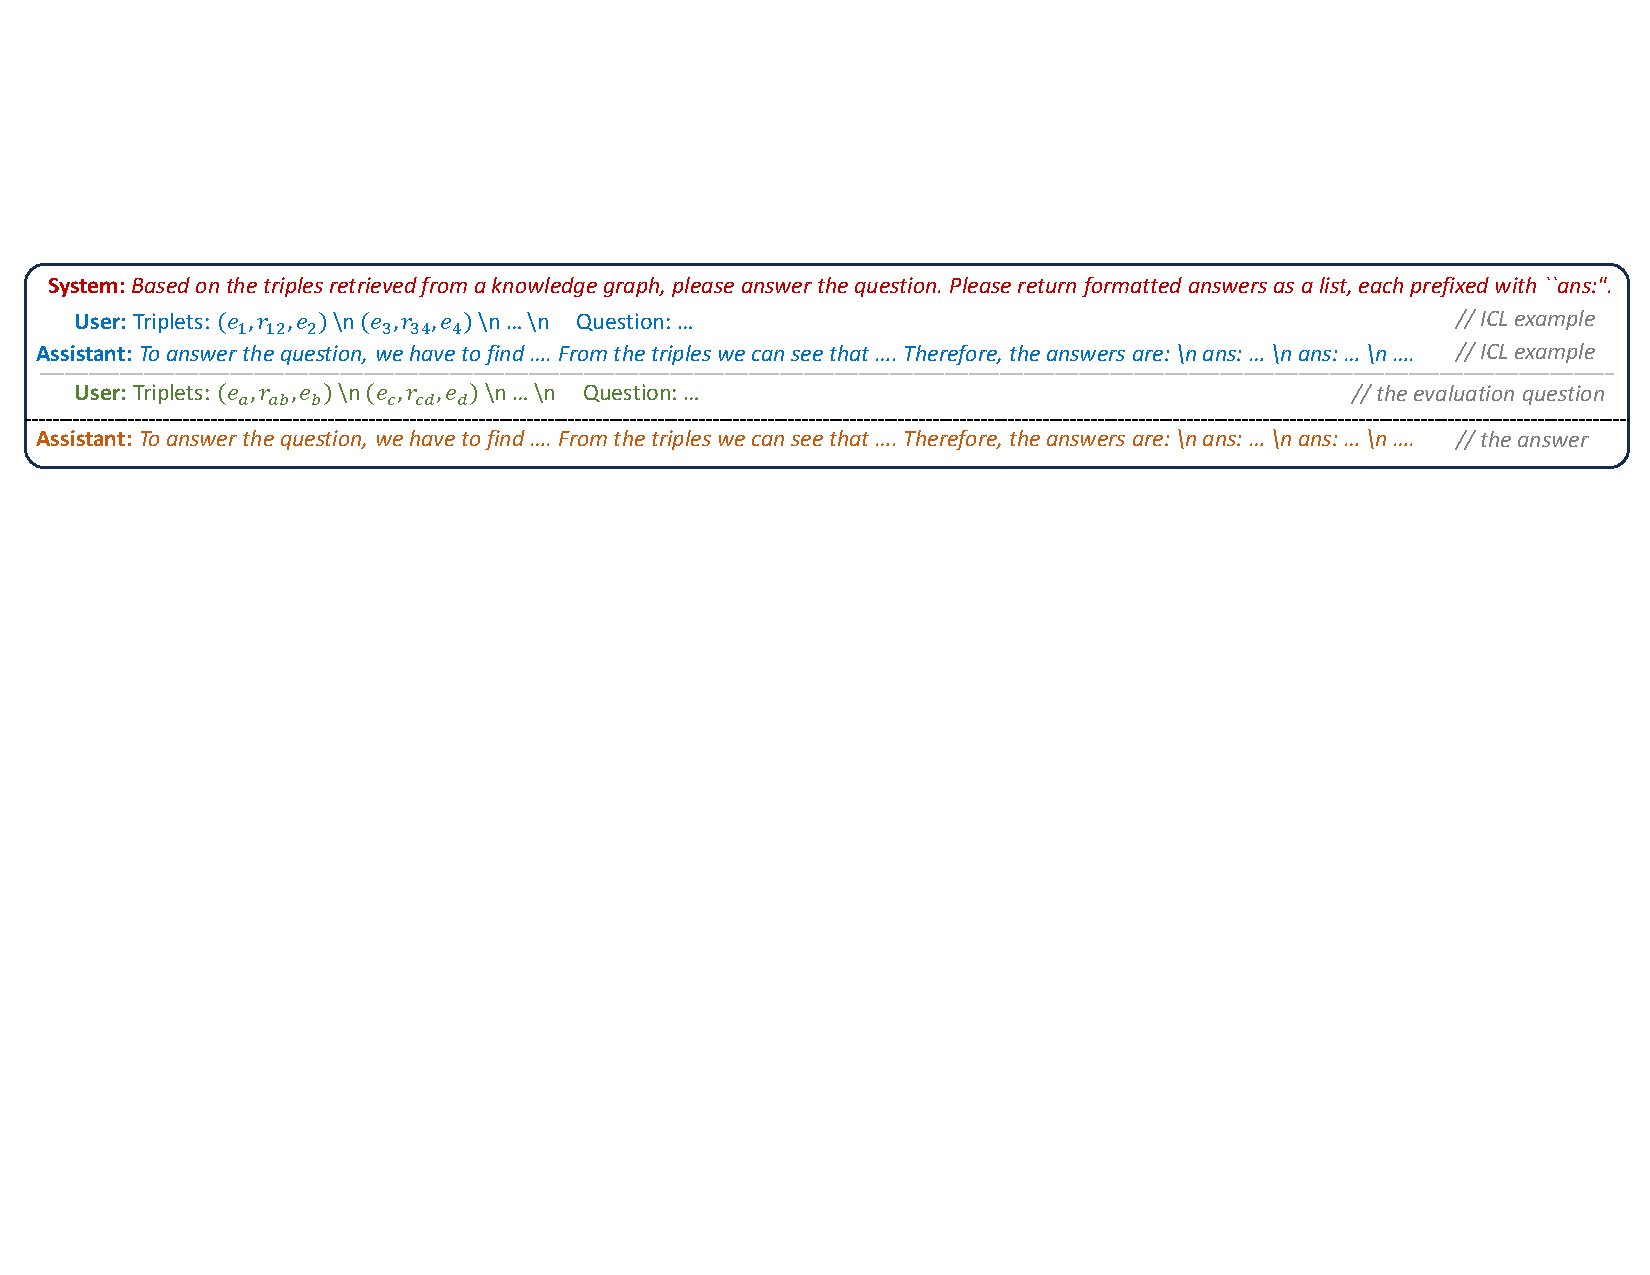
\includegraphics[trim={0.4cm 13.6cm 0.3cm 4.4cm},clip, width=\linewidth]{figs/prompt-format.pdf}
    \vspace{-7mm}
    \caption{The prompt used in \proj. Concrete examples can be found in Appendix~\ref{appendix:prompt}).
    \vspace{-6mm}
    \label{fig:prompt}}
\end{figure}


\subsection{Prompting-Based LLM Reasoning}

We employ an LLM to reason over $\gG_q$ by incorporating the linearized list of triples forming $\gG_q$ into the prompt. This approach allows the LLM to ground its reasoning in the retrieved structured knowledge and select the answers $\hat{\mathcal{A}}_{q}$ from the entities within $\gG_q$, mitigating issues like hallucinations and outdated knowledge~\citep{lin2019kagnet, shuster-etal-2021-retrieval-augmentation, vu-etal-2024-freshllms}. Specifically, we prompt the LLM to generate knowledge-grounded explanations besides the answers, which further effectively reduces hallucinations. We adopt in-context learning (ICL)~\citep{NEURIPS2020_1457c0d6}  and design dedicated prompt templates with explanation demonstrations to guide LLM reasoning (see Fig.~\ref{fig:prompt}).

Without fine-tuning LLMs, we reduce computational costs, enable the usage of state-of-the-art (SOTA) black-box LLMs, and maintain the generalizability for unseen KGs. Fine-tuning also risks enhancing prediction accuracy at the cost of general reasoning and explaining capabilities. High-quality text-based explanations are typically unavailable for question-answering tasks in practice. As a result, previous KG-based RAG approaches that rely on fine-tuning often depend on larger, unfine-tuned LLMs like GPT-4 to generate explanations as additional training data~\citep{luo2024rog}.

Regarding the size $K$ of the retrieved subgraph, while increasing $K$ in principle improves the coverage of relevant information, it also risks introducing more irrelevant information that may harm LLM reasoning~\citep{xu2024retrieval, liu-etal-2024-lost}. Different LLMs are inherently equipped with different sized context windows and also exhibit distinct capabilities in reasoning over long-context retrieval results~\citep{dubey2024llama3herdmodels}. As such, although the training of \proj retriever is LLM-agnostic, the size $K$ needs to be properly selected per LLM and constraints. In Section~\ref{para: reasoner_vary_k}, we empirically verify that more powerful LLMs can benefit from incorporating a larger-sized retrieved subgraph, demonstrating the benefit of size-adjustable subgraph retrieval in \proj.

% \subsection{More Related Works}

% Along with the introduction of \proj components, we have introduced the most relevant works. Other relevant works are reviewed in Appendix~\ref{appendix: related} due to the page limitation.
